\documentclass{article}
 
% Load the package
\usepackage{tikz}
\usepackage{tabularx}
\usepackage{forest} % https://ftp.agdsn.de/pub/mirrors/latex/dante/graphics/pgf/contrib/forest/forest-doc.pdf
\usepackage{amsfonts}

\usetikzlibrary{
    arrows,
    backgrounds,
    calc,
    %chains,
    decorations.pathreplacing,
    %decorations.pathmorphing,
    %matrix,
    %node-families,
    %positioning,
    %positioning-plus,
    shapes,
    %shapes.geometric,
    %shapes.symbols,
    topaths,
    %trees,
}

 
\begin{document}

\tikzstyle{texto} = [above, text width=6em, text centered]
% \newcommand{\fourup}[5]{%
%   \begin{pgfonlayer}{background}
%     % Left-top corner of the background rectangle
%     \path (#1.west |- #2.north)+(-0.5,0.5) node (a1) {};
%     % Right-bottom corner of the background rectanle
%     \path (#3.east |- #4.south)+(+0.5,-0.25) node (a2) {};
%     % Draw the background
%     \path[fill=yellow!20,rounded corners, draw=black!50, dashed]
%       (a1) rectangle (a2);
%     \path (a1.east |- a1.south)+(0.8,-0.3) node (u1)[texto]
%       {\scriptsize\textit{#5}};
%   \end{pgfonlayer}}
%   \newcommand{\threeup}[4]{%
%   \begin{pgfonlayer}{background}
%     % Left-top corner of the background rectangle
%     \path (#1.west |- #2.north)+(-0.5,0.5) node (a1) {};
%     % Right-bottom corner of the background rectanle
%     \path (#2.east |- #3.south)+(+0.5,-0.25) node (a2) {};
%     % Draw the background
%     \path[fill=yellow!20,rounded corners, draw=black!50, dashed]
%       (a1) rectangle (a2);
%     \path (a1.east |- a1.south)+(0.8,-0.3) node (u1)[texto]
%       {\scriptsize\textit{#4}};
%   \end{pgfonlayer}}
%   \newcommand{\twoup}[3]{%
%   \begin{pgfonlayer}{background}
%     % Left-top corner of the background rectangle
%     \path (#1.west |- #2.north)+(-0.5,0.5) node (a1) {};
%     % Right-bottom corner of the background rectanle
%     \path (#1.east |- #2.south)+(+0.5,-0.25) node (a2) {};
%     % Draw the background
%     \path[fill=yellow!20,rounded corners, draw=black!50, dashed]
%       (a1) rectangle (a2);
%     \path (a1.east |- a1.south)+(0.8,-0.3) node (u1)[texto]
%       {\scriptsize\textit{#3}};
%   \end{pgfonlayer}}

%%%%%%%%%%%%%%%%%%%%%%%%%%%%%%%%%%%%%
\section*{Introduction}

\renewcommand{\dots}{\ \dotfill{}\ } 
\newcommand{\command}[2]{#1~\dotfill{}~#2\\} 
\newcommand{\defin}[2]{#1~\dotfill{}~#2\\} 

\subsection{Graph maths}

\defin{Graph}{$G=(N,E)$}

\subsection{Graph implementations}
			
\subsection{Graph Algorithms}
			
\defin{BFS}{Breadth-first search}
\defin{DFS}{Depth-first search}
\defin{Random Walk}{randomize decision to follow edges}
\defin{Biased 2nd order Random Walk}{randomize decision to follow edges}

\subsection{Graph ML concepts}

\defin{note2vec}{Use flexible, biased random walks that can trade off between local and global views of the network\cite{grovlesk16}}
\defin{deepwalk}{...}

\subsection{Maths stuff}

\defin{Real numbers}{R}
\defin{Integers}{Z}

\subsection{Machine Learning concepts}

\defin{Stochastic Gradient Descent}{evaluate gradients for each individual training example}

\subsection{Machine Learning functions}

\defin{SoftMax}{$\sigma(z_i) = \frac{e^{z_{i}}}{\sum_{j=1}^K e^{z_{j}}} \ \ \ for\ i=1,2,\dots,K$}
\defin{Sigmoid}{$\sigma(z) = \frac{1} {1 + e^{-z}}$}
\defin{Relu}{$Relu(z) = max(0, z)$}
\defin{Mean Absolute Error (MAE)}{$\sum_{i=1}^{D}|x_i-y_i|$}
\defin{Mean Squared Error (MSE)}{$\sum_{i=1}^{D}(x_i-y_i)^2$}
%\defin{Huber loss}{$L_{\delta}=
%    \left\{\begin{matrix}
%        \frac{1}{2}(y - \hat{y})^{2} & if \left | (y - \hat{y})  \right | < \delta\\
%        \delta ((y - \hat{y}) - \frac1 2 \delta) & otherwise
%    \end{matrix}\right.$}
\defin{Cross Entropy}{$-{(y\log(p) + (1 - y)\log(1 - p))}$ for $M = 2$ \\ $-\sum_{c=1}^My_{o,c}\log(p_{o,c})$ for $M > 2$}    
					
\subsection{Statistics}

%\begin{tabular}{c >{\bfseries}r @{\hspace{0.7em}}c @{\hspace{0.4em}}c @{\hspace{0.7em}}l}
 % \multirow{10}{*}{\rotatebox{90}{\parbox{1.1cm}{\bfseriescentering actual value}}} & 
%    & \multicolumn{2}{c}{\bfseries Prediction outcome} & 
%  & & \bfseries p & \bfseries n & \bfseries total 
%  & p$'$ & \MyBox{True}{Positive} & \MyBox{False}{Negative} & P$'$ [2.4em]
%  & n$'$ & \MyBox{False}{Positive} & \MyBox{True}{Negative} & N$'$ 
%  & total & P & N &
%\end{tabular}

\defin{True Positive}{$TP$}
\defin{False Positive}{$FP$}
\defin{True Negative}{$TN$}
\defin{False Negative}{$FN$}
\defin{Precision}{$\frac{TP}{TP+FP}$}
\defin{Recall}{$\frac{TP}{TP+FN}$}
\defin{Accuracy}{$\frac{TP+TN}{TP+TN+FP+FN}$}
\defin{Sensitivity = Recall}{$\frac{TP}{TP+FN}$}
\defin{Specificity}{$\frac{TN}{FP+TN}$}
\defin{Cosine similarity}{$Cosine(x,y) = \frac{x \cdot y}{|x||y|}$}
\defin{Jaccard similarity}{$Jaccard(U,V) = \frac{|U \cap V|}{|U \cup V|}$}
\defin{Pointwise Mutual Information (PMI) similarity}{$PMI(x;y) = \log{\frac{p(x,y)}{p(x)p(y)}}$}


\section{Over-smoothing}

This problem happens when we stack too many layers in a GNN. The 
problem is that the embeddings tend to converge to a similar value. 
But we want node embeddings to be different.

The problem is that as we go out from the node of interest, the number of 
shared nodes also goes up. The embedding of a node is determined by the \emph{receptive field}. A receptive field is a set of nodes that are connected to the node of interest. If two nodes have highly overlapping receptive fields, then the embeddings will be likewise very similar. This results in the over-smoothing problem.

\subsubsection{Layers}

We need to be careful we don't have too many layers. A too deep network will result in oversmoothing. Setting the number of layers to be only slightly more than the size of the receptive field is a good first approximation.

\subsubsection{Increase expressive power}

One approach is to increase expressive power with each layer.

\begin{figure}[ht]
    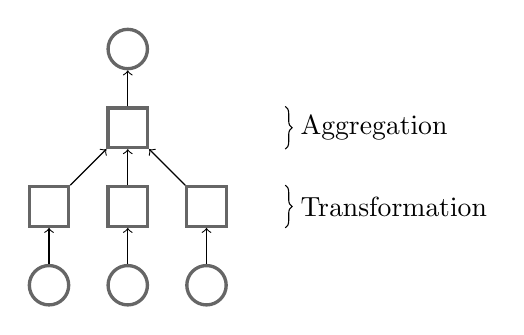
\begin{tikzpicture}[
        layer/.style={rectangle, draw=black!60, fill=white, very thick, minimum size=5mm},
        inout/.style={circle, draw=black!60, fill=white, very thick, minimum size=5mm},
        layergroup/.style={decorate},
        tubnode/.style={midway, right=2pt},
        ]
        \node[inout] (OUT)              {}; 
        \node[layer] (AGG) [below of=OUT] {}; 
        \node[layer] (TR2) [below of=AGG] {}; 
        \node[layer] (TR1) [left of=TR2] {}; 
        \node[layer] (TR3) [right of=TR2] {}; 
        \node[inout] (IN1) [below of=TR1] {}; 
        \node[inout] (IN2) [below of=TR2] {}; 
        \node[inout] (IN3) [below of=TR3] {}; 
        \draw[->] (AGG) -- (OUT);
        \draw[->] (TR1) -- (AGG); 
        \draw[->] (TR2) -- (AGG); 
        \draw[->] (TR3) -- (AGG); 
        \draw[->] (IN1) -- (TR1); 
        \draw[->] (IN2) -- (TR2); 
        \draw[->] (IN3) -- (TR3);
        \draw[layergroup, decoration={brace}] let \p1=(AGG.north), \p2=(AGG.south) in
        ($(2, \y1)$) -- ($(2, \y2)$) node[tubnode] {Aggregation};
        \draw[layergroup, decoration={brace}] let \p1=(TR2.north), \p2=(TR2.south) in
        ($(2, \y1)$) -- ($(2, \y2)$) node[tubnode] {Transformation};    
    \end{tikzpicture}
    \caption{A simple GNN}
\end{figure}

In both the aggregation and transformation layers, we could include a 3-layer MLP.  

\subsubsection{Adding non-message passing layers}

We can add pre- and postprocessing layers. See \ref{sec:simple-gnn}.

\begin{figure}[h]
    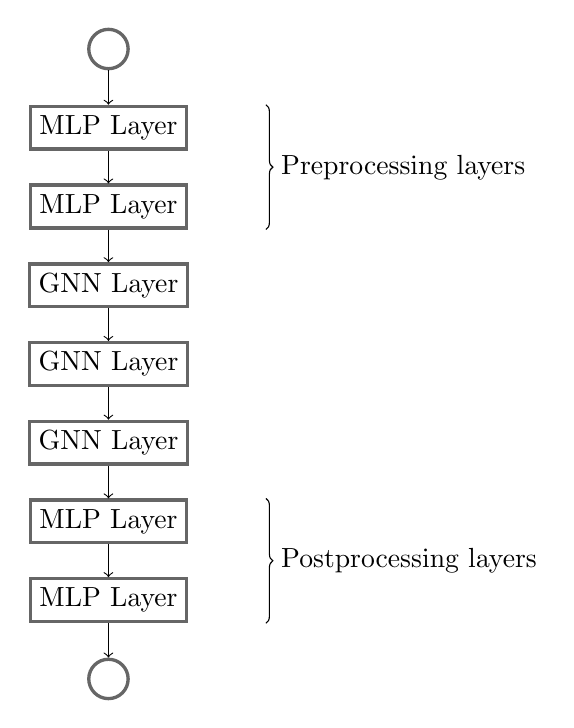
\begin{tikzpicture}[
        layer/.style={rectangle, draw=black!60, fill=white, very thick, minimum size=5mm},
        layergroup/.style={decorate},
        tubnode/.style={midway, right=2pt},
        inout/.style={circle, draw=black!60, fill=white, very thick, minimum size=5mm},
        ]
        \node[inout] (IN)                   {}; 
        \node[layer] (MLP1) [below of=IN]   {MLP Layer}; 
        \node[layer] (MLP2) [below of=MLP1] {MLP Layer}; 
        \node[layer] (GNN3) [below of=MLP2] {GNN Layer}; 
        \node[layer] (GNN4) [below of=GNN3] {GNN Layer}; 
        \node[layer] (GNN5) [below of=GNN4] {GNN Layer}; 
        \node[layer] (MLP6) [below of=GNN5] {MLP Layer}; 
        \node[layer] (MLP7) [below of=MLP6] {MLP Layer}; 
        \node[inout] (OUT)  [below of=MLP7] {}; 
        \draw[->] (IN) -- (MLP1); 
        \draw[->] (MLP1) -- (MLP2); 
        \draw[->] (MLP2) -- (GNN3); 
        \draw[->] (GNN3) -- (GNN4); 
        \draw[->] (GNN4) -- (GNN5); 
        \draw[->] (GNN5) -- (MLP6); 
        \draw[->] (MLP6) -- (MLP7); 
        \draw[->] (MLP7) -- (OUT); 
        \draw[layergroup, decoration={brace}] let \p1=(MLP1.north), \p2=(MLP2.south) in
        ($(2, \y1)$) -- ($(2, \y2)$) node[tubnode] {Preprocessing layers};
        \draw[layergroup, decoration={brace}] let \p1=(MLP6.north), \p2=(MLP7.south) in
        ($(2, \y1)$) -- ($(2, \y2)$) node[tubnode] {Postprocessing layers};
        %\twoup{MLP1}{MLP2}{Preprocessing layers};
        %\threeup{GNN3}{GNN4}{GNN5}{group};
        %\twoup{MLP6}{MLP7}{Preprocessing layers};
    
    \end{tikzpicture}
    \caption{A simple GNN}
    \label{fig:simple-gnn}
\end{figure}

These MLP layers refine the features of the nodes before and after the GNN layers. The preprocessing layers could process note features, for instance, if the nodes represent images or text. The postprocessing layers could process the embedding, for instance, if we want to use the embedding as a feature for classification.
    
\subsubsection{Skip Connections}
Skip the layers in the neural Network. See \ref{fig:simpleskipping}

\begin{figure}[h]
    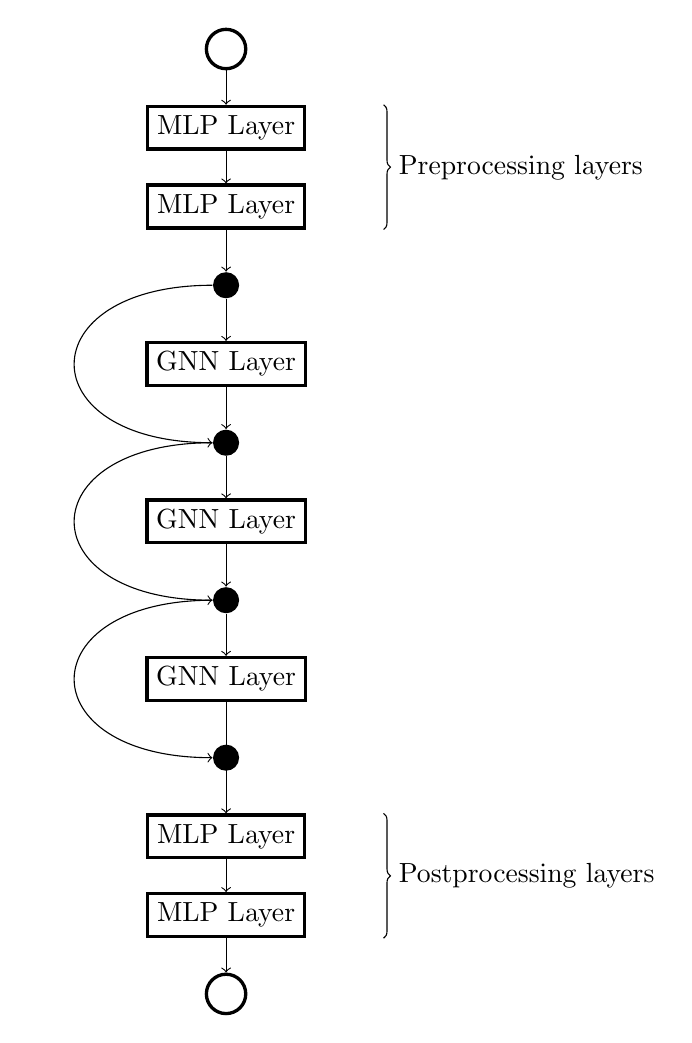
\begin{tikzpicture}[
        layer/.style={rectangle, draw=black, fill=white, very thick, minimum size=5mm},
        layergroup/.style={decorate},
        tubnode/.style={midway, right=2pt},
        inout/.style={circle, draw=black, fill=white, very thick, minimum size=5mm},
        silent/.style={circle,fill=black,minimum size=1pt}
        ]
        \node[inout]  (IN)                     {};
        \node[layer]  (MLP11) [below of=IN]    {MLP Layer};
        \node[layer]  (MLP12) [below of=MLP11] {MLP Layer};
        \node[silent] (S1)    [below of=MLP12] {};
        \node[layer]  (GNN1)  [below of=S1]    {GNN Layer}; 
        \node[silent] (S2)    [below of=GNN1]  {};
        \node[layer]  (GNN2)  [below of=S2]    {GNN Layer};
        \node[silent] (S3)    [below of=GNN2]  {};
        \node[layer]  (GNN3)  [below of=S3]    {GNN Layer}; 
        \node[silent] (S4)    [below of=GNN3]  {};
        \node[layer]  (MLP21) [below of=S4]    {MLP Layer}; 
        \node[layer]  (MLP22) [below of=MLP21] {MLP Layer}; 
        \node[inout]  (OUT)   [below of=MLP22]  {}; 
        \draw[->] (IN) -- (MLP11); 
        \draw[->] (MLP11) -- (MLP12); 
        \draw[->] (MLP12) -- (S1); 
        \draw[->] (S1) -- (GNN1); 
        %\draw[->] (MLP2) -- (GNN4);
        \draw[->] (S1) to [out=-180,in=180,looseness=3] (S2); 
        \draw[->] (GNN1) -- (S2); 
        \draw[->] (S2) -- (GNN2);
        \draw[->] (S2) to [out=-180,in=180,looseness=3] (S3); 
        \draw[->] (GNN2) -- (S3); 
        \draw[->] (S3) -- (GNN3);
        \draw[->] (S3) to [out=-180,in=180,looseness=3] (S4); 
        \draw[->] (GNN3) -- (MLP21);
        \draw[->] (MLP21) -- (MLP22); 
        \draw[->] (MLP22) -- (OUT); 
        \draw[layergroup, decoration={brace}] let \p1=(MLP11.north), \p2=(MLP12.south) in
        ($(2, \y1)$) -- ($(2, \y2)$) node[tubnode] {Preprocessing layers};
        \draw[layergroup, decoration={brace}] let \p1=(MLP21.north), \p2=(MLP22.south) in
        ($(2, \y1)$) -- ($(2, \y2)$) node[tubnode] {Postprocessing layers};
        %\twoup{MLP1}{MLP2}{Preprocessing layers};
        %\threeup{GNN3}{GNN4}{GNN5}{group};
        %\twoup{MLP6}{MLP7}{Preprocessing layers};
    
    \end{tikzpicture}
    \caption{A simple GNN with skipping}
    \label{fig:simpleskipping}
\end{figure}


% \begin{tikzpicture}[node distance={15mm}, thick, main/.style = {draw, circle}] 
% \node[main] (1) {$x_1$}; 
% \node[main] (2) [above right of=1] {$x_2$}; 
% \node[main] (3) [below right of=1] {$x_3$}; 
% \node[main] (4) [above right of=3] {$x_4$}; 
% \node[main] (5) [above right of=4] {$x_5$}; 
% \node[main] (6) [below right of=4] {$x_6$}; 
% \draw[->] (1) -- (2); 
% \draw[->] (1) -- (3); 
% \draw (1) to [out=135,in=90,looseness=1.5] (5); 
% \draw (1) to [out=180,in=270,looseness=5] (1); 
% \draw (2) -- (4); 
% \draw (3) -- (4); 
% \draw (5) -- (4); 
% \draw[->] (5) to [out=315, in=315, looseness=2.5] (3); 
% \draw[->] (6) -- node[midway, above right, sloped, pos=1] {+1} (4); 
% \end{tikzpicture} 
 
 

\section{A general GNN framework}

Comprised of layers of transformers and aggregators where messages are being passed between the layers. The transformers are used to process the input data and the aggregators are used to combine the output of the transformers.

\section{Graph augmentation}

The raw input graph may not be the same as the computational graph. We use \emph{graph feature} and \emph{graph structure} augmentation.

\subsection{Graph feature augmentation}

Sometimes, nodes don't have features. We could just assign a constant value to each node. This isn't as dumb as it sounds as it still allows the node to be described by it's connections to other nodes.

We could also use a \emph{one-hot} encoding for each node. This is a simple way to encode the node's feature. For a six node graph, we could use a vector of length six with a one at the index of the node, like $\textit{id}_5 = [0,0,0,0,1,0]$. However, it might be hard to generalize this encoding if the node numbers are arbitrary.

\subsection*{Comparing constant to one-hot encoding}
%\begin{table}[h]
\begin{tabularx}{\textwidth}{XXX}
    \hline \hline 
     & Constant node feature & One-hot node feature \\
    Expressive Power & Medium. All the nodes are identical, but GNN can still learn from the graph structure & High. Each node has a unique ID, so node-specific information can be stored \\
    Inductive learning (Generalize to unseen models) & High. Simple to generalize to nodes: we assign constant feature to them, then apply our GNN & Low. Cannot generalize to new nodes: new nodes introduce new IDs, GNN doesn't know how to embed unseen IDs. \\
    Computational cost & Low. Ony one dimensional feature & high. $O(|V|)$ dimensional feature cannot apply to large graphs. \\
    Use cases & Any graph, unductive settings (generalize to new nodes) & Small graph, transductive settings (no new nodes) \\
    \hline \hline 
\end{tabularx}
%\end{table}

\subsection{Hard to learn structures}

Sometimes, the structures are hard for the GNN to learn. For examples, cycles are often a problem.

$v_1$ resides in a cycle with length 3:

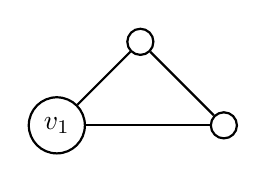
\begin{tikzpicture}[node distance={15mm}, thick, main/.style = {draw, circle}] 
\node[main] (1) {$v_1$}; 
\node[main] (2) [above right of=1] {}; 
\node[main] (3) [below right of=2] {}; 
\draw (1) -- (2); 
\draw (2) -- (3); 
\draw (3) -- (1); 
\end{tikzpicture} 

$v_1$ resides in a cycle with length 4:

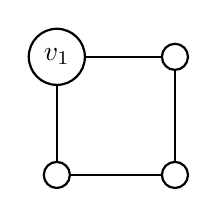
\begin{tikzpicture}[node distance={15mm}, thick, main/.style = {draw, circle}] 
    \node[main] (1) {$v_1$}; 
    \node[main] (2) [right of=1] {}; 
    \node[main] (3) [below of=2] {}; 
    \node[main] (4) [below of=1] {}; 
    \draw (1) -- (2); 
    \draw (2) -- (3); 
    \draw (3) -- (4); 
    \draw (4) -- (1); 
\end{tikzpicture} 

$v_1$ resides in a cycle with infinite length:


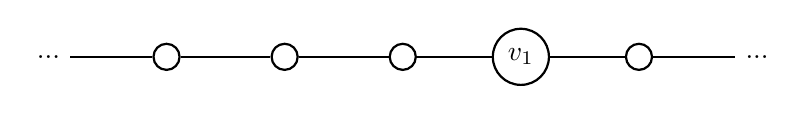
\begin{tikzpicture}[node distance={15mm}, thick, main/.style = {draw, circle}] 
    \node       (1)              {...}; 
    \node[main] (2) [right of=1] {};
    \node[main] (3) [right of=2] {};
    \node[main] (4) [right of=3] {}; 
    \node[main] (5) [right of=4] {$v_1$}; 
    \node[main] (6) [right of=5] {}; 
    \node (7)       [right of=6] {...}; 
    \draw (1) -- (2); 
    \draw (2) -- (3); 
    \draw (3) -- (4); 
    \draw (4) -- (5); 
    \draw (5) -- (6); 
    \draw (6) -- (7); 
\end{tikzpicture} 

Those are virtually the same as this for a GNN. The computational graph is always the same for these:

% see: https://ftp.agdsn.de/pub/mirrors/latex/dante/graphics/pgf/contrib/forest/forest-doc.pdf
\begin{forest}
    for tree={circle,draw, l sep=20pt}
    [$v_1$ 
        [.  
          [.
            [.]
            [.]
          ] 
          [.
            [.]
            [.]
          ]
        ]
        [.  
          [.
            [.]
            [.]
          ] 
          [.
            [.]
            [.]
          ]
        ]
    ]
\end{forest}
    

A possible solution would be to create features that reflect the structure.

\begin{itemize}
	\item Features could include
	\item node dgree
	\item clustering coefficient
	\item pagerank
	\item centrality
	\item ... (anything we know about from classical graph theory)
\end{itemize}

\subsection{Graph structure augmentation}

Motivation augment sparse graphs.

\subsubsection{Add virtual edges}

. For instance, connect 2-hop neighbors via virtual edges. Intuition entrad of using adjacency matrix A for GNN computation, use $A + A^2$.

Use cases: bibartite graphs like author-to-papers or 2-hop virtual edges to make author-author collaboration graph.

\subsubsection{Add Virtual nodes}

Intuition: connect nodes that are far apart and make the message passing more efficient.

\subsubsection{What if we have too many nodes?}

Intuition: randomly sample a fraction of the nodes connected to the node under observation. We gain computational efficiency, but may lose expressiveness.

This works particular well in graphs with large fanout/in. 

\section{Training a GNN}

Roughly:

\begin{enumerate}
    \item Start with input graph
    \item create the Graph Neural Network
    \item Find the Node embeddings
    \item Prediction Head
    \item Predictions (to Loss function and Evaluation metrics)
    \item Loss function
    \item Evaluation Metrics
    \item Labels (to Loss function and Evaluation metrics)
\end{enumerate}

\subsection{Prediction Head}

output of the GNN.

Node level prediction: we can directly make predictions using the node embeddings. After the GNN computation, we have $d-dim$ node embeddings: $\{h_v^{(L)} \in \mathbb{R}^d, \forall v \in G\}$.
We might want to classify the nodes into $k$ classes. We need to make the node embeddings $h_v^{(L)} \in \mathbb{R}^d$ to the predictions $\hat{y}_v \in \mathbb{R}^k$. 

For edge-level tasks we need to consider pairs of nodes.
An approach is concatination and applying a linear function to get $\hat{y}_{uv}$. Or we could use the dot product: $\hat{y}_{uv} = (h_u^{(L)})^T h_v^{(L)}$. This can only predict the existence of an edge, so just one-way. K-way prediction is similar to multi-head attention. 

$\hat{y}_{uv}^{(k)} = (h_u^{(L)})^TW^{(1)}h_v^{(L)}$

$\hat{y}_{uv} = Concat(\hat{y}_{uv}^{(k)} \forall k) \in \mathbb{R}$

Graph-level predictions: We need to take the node embeddings and somehoe combine them into a graph level prediction.

\begin{enumerate}
    \item Gobal mean pooling: $\hat{y}_G = Mean(\{h_v^{(L)} \in \mathbb{R}^d, \forall v \in G \})$.
    \item Global max pooling:$\hat{y}_G = Max(\{h_v^{(L)} \in \mathbb{R}^d, \forall v \in G \})$.
    \item Global sum pooling:$\hat{y}_G = Sum(\{h_v^{(L)} \in \mathbb{R}^d, \forall v \in G \})$.
\end{enumerate}

These are OK on small graphs. But Global pooling over a large graphs loses a lot of information. Instead, we can used hierarchical pooling. 
In effect, we are splitting the graph into communities that we evaluate and then aggregrate to get to the prediction head. The partitioning can be learned \cite{DiffPool}.

\subsection{predictions}

We talk about, \emph{supervised} and \emph{unsupervised} (AKA \emph{self-supervised}).

\subsubsection{Supervised labels on graphs}

\begin{itemize}
    \item Node labels $y_v$: E.g., in a citation network, which subject area does a node belong to
    \item Edge labels $y_{uv}$: E.g., in a transaction network,whether an edge is fraudulent
    \item Graph labels $y_G$: E.g., among molecular graphs, the drug likeness of graphs
\end{itemize}

Try to formulate your task as one of these so that reusing this research can benefit us.

\subsubsection{unsupervised labeles on graphs}

\begin{itemize}
    \item Node-level $y_v$: Node statistics such as clustering coefficient, degree, Pagerank, etc.
    \item Edge-level $y_{uv}$: Link prediction hide the edge between two nodes, then predict there should be a link.
    \item Graph-level $y_G$: Graph statistics such as predict if two graphs are isomorphic
\end{itemize}

\subsection{Loss function}

Given $N$ data points:

\begin{itemize}
    \item Node-level: prediction $\hat{y}_v^{(i)}$, label $y_v^{(i)}$
    \item Edge-level: prediction $\hat{y}_{uv}^{(i)}$, label $y_{uv}^{(i)}$
    \item Graph-level: prediction $\hat{y}_G^{(i)}$, label $y_G^{(i)}$
    \item Prediction $\hat{y}^{(i)}$, label $y^{(i)}$ refers to all levels
\end{itemize}

\begin{itemize}
    \item Classification: labels $y^{(i)}$ with discrete value: What category does a (something) belong to.
    \item Regression: labels $y^{(i)}$ with continuous value: What is the likliness of a (something).
\end{itemize}

These will need different loss functions and evaluation metrics.

\subsubsection{Cross entropy}

This is a very common loss function.

$CE(y^{(i)}, \hat{y}^{(i)}) = -\sum_{j=1}^K y_j^{(i)} \log(\hat{y}_j^{(i)})$ with the i-th data point and j-th target.

Where,

$y^{(i)} \in \mathbb{R}^K =$ one-hot label encoding. E.g.,

\begin{tabular}{|c|c|c|c|c|}
    \hline
    0 & 0 & 1 & 0 & 0 \\
    \hline    
\end{tabular}

$\hat{y}^{(i)} \in \mathbb{R}^K =$ predicted one-hot label encoding after Softmax.

\begin{tabular}{|c|c|c|c|c|}
    \hline
    0.1 & 0.3 & 0.4 & 0.1 & 0.1 \\
    \hline    
\end{tabular}

(Note: predicted values are probabilities and must add up to $1.0$.)

What we are looking for is to match the predictions to the labeling. The highest probability is the one that matches the label.

The total loss over all N training examples is:

$Loss = \sum_{i=1}^N CE(y^{(i)}, \hat{y}^{(i)})$


\subsubsection{Mean square Error}

For Regression tasks we can use \emph{Mean Squared Error} (MSE) loss function AKA \emph{L2 loss}.

useful for finding node ordering, rather than classification

K-way regression for data point $(i)$:

$\mathit{MSE}(y^{(i)}, \hat{y}^{(i)}) = -\sum_{j=1}^K (y_j^{(i)} - \hat{y}_j^{(i)})^2$ with the i-th data point and j-th target.

Where,

$y^{(i)} \in \mathbb{R}^K =$ Real-valued vector of targets. E.g.,

\begin{tabular}{|c|c|c|c|c|}
    \hline
    1.4 & 2.3 & 1.0 & 0.5 & 0.6 \\
    \hline    
\end{tabular}

$\hat{y}^{(i)} \in \mathbb{R}^K =$ Real valued vector of predictions. E.g.,

\begin{tabular}{|c|c|c|c|c|}
    \hline
    0.9 & 2.8 & 2.0 & 0.3 & 0.8 \\
    \hline    
\end{tabular}

The total loss over all N training examples is:

$Loss = \sum_{i=1}^N MSE(y^{(i)}, \hat{y}^{(i)})$ 


\subsection{Evaluation metrics}

RMSE: Root Mean Square Error

$RMSE(y^{(i)}, \hat{y}^{(i)}) = \sqrt{\frac{1}{N} \sum_{i=1}^N (y^{(i)} - \hat{y}^{(i)})^2}$

MAE: Mean Absolute Error

$MAE(y^{(i)}, \hat{y}^{(i)}) = \frac{1}{N} \sum_{i=1}^N |y^{(i)} - \hat{y}^{(i)}|$


\clearpage


\begin{thebibliography}{10}

  \bibitem{grovlesk16} Grover and Leskovovec, 
  \emph{???}, 2016.
  
  \bibitem{latexMath} Graetzer George, \emph{Math Into \LaTeX},
  Birkuser Boston; 3 edition (June 22, 2000).
  
\end{thebibliography}
  
\end{document}
